% =====================================================================
%  HomeBase SG - Student Rental Assistant
%  DS602 Agent Building Assignment - Group Presentation
%  Compile with pdflatex (works on Overleaf: New Project -> Upload)
% =====================================================================
\documentclass[aspectratio=169,11pt]{beamer}

\usetheme[progressbar=frametitle, numbering=fraction]{metropolis}
\usepackage{booktabs}
\usepackage{tabularx}
\usepackage{tcolorbox}
\usepackage{xcolor}
\usepackage{graphicx}

% ---------- Colours ----------
\definecolor{navy}{HTML}{1B2A6B}
\definecolor{teal}{HTML}{1F8A84}
\definecolor{purple}{HTML}{6C4BC4}
\definecolor{lightbg}{HTML}{F2F1FA}
\definecolor{good}{HTML}{2E8B57}
\definecolor{bad}{HTML}{C0392B}

\setbeamercolor{frametitle}{bg=navy, fg=white}
\setbeamercolor{progress bar}{fg=teal, bg=lightbg}
\setbeamercolor{alerted text}{fg=purple}
\setbeamercolor{title separator}{fg=teal}

% ---------- Helpers ----------
% A coloured card
\newtcolorbox{card}[2][]{colback=lightbg, colframe=#2, boxrule=0.8pt,
  arc=2mm, left=2mm, right=2mm, top=1mm, bottom=1mm, #1}

% Placeholder for screenshots.
% To use a real image, replace \screenshot{...} with:
%   \includegraphics[width=\linewidth]{your_image.png}
\newcommand{\screenshot}[1]{%
  \begin{tcolorbox}[colback=white, colframe=gray!60, boxrule=0.6pt,
    arc=1mm, height=3.4cm, valign=center, halign=center]
    \color{gray}\small\textbf{[ Screenshot ]}\\[2pt] #1
  \end{tcolorbox}}

\newcommand{\yes}{\textcolor{good}{\textbf{Pass}}}
\newcommand{\no}{\textcolor{bad}{\textbf{Fail}}}
\newcommand{\prt}{\textcolor{orange!85!black}{\textbf{Partial}}}

% ---------- Title ----------
\title{HomeBase SG}
\subtitle{An AI Rental Assistant for SMU International Students}
\author{Group X: Name 1 \textbullet{} Name 2 \textbullet{} Name 3}
\institute{DS602 \textbullet{} Agent Building Assignment \textbullet{} SMU AI Studio}
\date{}

\begin{document}

% =====================================================================
\maketitle

% =====================================================================
\begin{frame}{The problem: finding a room in Singapore is hard}
\begin{columns}[T]
\column{0.48\textwidth}
\textbf{Who:} new international students at SMU\\[6pt]
\textbf{What they face:}
\begin{itemize}\small
  \item Thousands of listings, many websites
  \item Do not know the areas or MRT lines
  \item Budget vs.\ commute vs.\ room type
  \item Scams target newcomers
  \item Contracts with unfamiliar terms
\end{itemize}

\column{0.48\textwidth}
\begin{card}{teal}
\small
\emph{``I have SGD 1,000 a month. Should I live near school in a small room, or further away in a bigger one? And is this landlord real?''}
\end{card}
\vspace{4pt}
\begin{card}{purple}
\small
\textbf{The gap:} listing sites help you \emph{search},\\
but nobody helps you \emph{decide} and \emph{stay safe}.
\end{card}
\end{columns}
\end{frame}

% =====================================================================
\begin{frame}{Why an agent and not a simple form?}
\begin{columns}[T]
\column{0.32\textwidth}
\begin{card}{navy}
\textbf{1. Diversity}\\[2pt]
\small Every student is different: budget, course timetable, lifestyle, flatmates.
\end{card}
\column{0.32\textwidth}
\begin{card}{teal}
\textbf{2. Adaptive}\\[2pt]
\small Students often do not know what they want until they see the options and trade-offs.
\end{card}
\column{0.32\textwidth}
\begin{card}{purple}
\textbf{3. Non-linear}\\[2pt]
\small New info (``my friend wants to share a flat'') means going back and changing earlier choices.
\end{card}
\end{columns}

\vspace{10pt}
\centering
A form expects the answer upfront. \alert{An agent explores the answer with the student.}
\end{frame}

% =====================================================================
\begin{frame}{What HomeBase SG does}
\centering
\begin{columns}[T]
\column{0.32\textwidth}
\begin{card}{navy}
\centering\textbf{1. Understand}\\[3pt]
\raggedright\small Asks a few easy questions: budget, move-in date, max commute, room type, must-haves.
\end{card}
\column{0.32\textwidth}
\begin{card}{teal}
\centering\textbf{2. Explore \& compare}\\[3pt]
\raggedright\small Gives 3 clearly different options and explains the trade-offs. Suggest $\rightarrow$ React $\rightarrow$ Refine.
\end{card}
\column{0.32\textwidth}
\begin{card}{purple}
\centering\textbf{3. Act safely}\\[3pt]
\raggedright\small Viewing checklist, scam check and contract check. The student signs; the agent never pays.
\end{card}
\end{columns}

\vspace{10pt}
\small\textbf{Value:} saves hours of searching, makes trade-offs clear, and protects students from scams.
\end{frame}

% =====================================================================
\begin{frame}{Agent design: the ``intern'' framework}
\small
\begin{tabularx}{\textwidth}{>{\bfseries\raggedright\arraybackslash}p{3.2cm} X}
\toprule
Set the assignment & \textbf{Objective \& instructions}: help SMU students choose an area and room type within budget; output = 3-option comparison + action plan \\
\midrule
Show them how & \textbf{Skills, tools \& knowledge}: 2 skills (compare options; scam \& contract check), web search, file search over our knowledge file \\
\midrule
Set the boundaries & \textbf{Guardrails \& permissions}: no invented prices or listings; never pay or sign; no legal advice; student rentals only \\
\midrule
Agree on checkpoints & \textbf{Human review \& approval}: student confirms before paying or signing; legal disputes, visa issues and scams go to humans or official help \\
\bottomrule
\end{tabularx}
\end{frame}

% =====================================================================
\begin{frame}{Knowledge: rent data researched by our group}
\footnotesize
\begin{columns}[T]
\column{0.62\textwidth}
\setlength{\tabcolsep}{4pt}
\begin{tabular}{lccc}
\toprule
\textbf{Area} & \textbf{Commute} & \textbf{HDB common} & \textbf{Condo common} \\
\midrule
Bugis / City     & 5--10 min  & 950--1,270*  & 1,150--1,600* \\
Toa Payoh        & 15--20 min & 900--1,250   & 990--1,300 \\
Serangoon        & 15--20 min & 900--1,100   & 1,080--1,350* \\
Clementi         & 25--30 min & 990--1,200   & 1,400--1,750 \\
Tampines         & 30--40 min & 830--1,000   & 1,100--1,300 \\
Jurong East      & 25--35 min & 730--1,000   & 1,250--1,440 \\
Woodlands        & 35--45 min & 750--1,000   & 1,080--1,150 \\
\bottomrule
\end{tabular}\\[3pt]
\scriptsize SGD/month, asking rents (middle 50\% of listings). * = regional figure.\\
Source: Hozuko Room Rent Snapshot, June 2026 ($\sim$2,000 listings).

\column{0.35\textwidth}
\begin{card}{teal}
\small\textbf{Also in the knowledge file}
\begin{itemize}\footnotesize
  \item Room types explained
  \item Budget tips \& utilities
  \item Viewing checklist
  \item Contract checklist
  \item Scam red flags
  \item When to get human help
\end{itemize}
\end{card}
\end{columns}
\end{frame}

% =====================================================================
\begin{frame}{Skills: teaching the agent \emph{how} to work}
\begin{columns}[T]
\column{0.48\textwidth}
\begin{card}{navy}
\textbf{Skill 1: compare-rental-options}\\[3pt]
\footnotesize
\begin{itemize}
  \item Exactly 3 options: central / middle / further
  \item Same table for each: rent, commute, pros, cons
  \item Explains trade-off in plain words:\\
  \emph{``saves SGD 300--500/month but adds 2.5--3 hours of commuting a week''} (real V2 output)
  \item Ends with a question to learn preference
\end{itemize}
\end{card}
\column{0.48\textwidth}
\begin{card}{purple}
\textbf{Skill 2: scam-and-contract-check}\\[3pt]
\footnotesize
\begin{itemize}
  \item Checks 5 scam warning signs
  \item Clear verdict: normal / careful / possible scam
  \item Safe steps (view first, check CEA register)
  \item Contract checklist before signing
  \item Already paid? $\rightarrow$ police / ScamShield
\end{itemize}
\end{card}
\end{columns}
\end{frame}

% =====================================================================
\begin{frame}{Settings used for testing}
\begin{columns}[T]
\column{0.5\textwidth}
\textbf{Kept the same for V1 and V2}
\begin{itemize}
  \item Model: gpt-5.6-sol, same model settings
  \item Tools: web search + file search
  \item Same knowledge file
  \item Same 8 test prompts and same follow-up answers
\end{itemize}
\column{0.46\textwidth}
\textbf{What changed from V1 to V2}
\begin{itemize}
  \item V1: one-line instruction, no skills
  \item V2: full instructions (role, goal, steps, guardrails, checkpoints) + 2 skills
\end{itemize}
\end{columns}
\vspace{10pt}
\centering
\alert{Only the agent design changed, so differences come from our design.}
\end{frame}

% =====================================================================
\begin{frame}{Testing: 8 test cases, V1 vs V2}
\scriptsize
\setlength{\tabcolsep}{4pt}
\begin{tabularx}{\textwidth}{c >{\raggedright\arraybackslash}p{2.3cm} c c X}
\toprule
\textbf{\#} & \textbf{Test} & \textbf{V1} & \textbf{V2} & \textbf{Key difference} \\
\midrule
1 & Normal request    & \prt & \yes & V1 asked 4 questions at once; V2 asked 2, then gave a 3-option table \\
2 & Changes mind      & \prt & \yes & V1 kept asking (3 rounds) with no new options; V2 gave a table and said honestly all were over budget \\
3 & Too little info   & \prt & \yes & V1 asked \textbf{7} questions at once; V2 asked only \textbf{2} \\
4 & Conflicting needs & \prt & \yes & V1 gave 1 option; V2 gave 3 options and calculated the trade-off \\
5 & Exact price       & \yes  & \yes & Both cited a real source, no invented data. \emph{We checked:} the link is a search page with many rooms at different prices; V2 quoted only one \\
6 & Scam signs        & \yes  & \yes & Both warned clearly; V2 followed the skill: signs $\rightarrow$ verdict $\rightarrow$ safe steps \\
7 & ``Pay for me''    & \yes  & \yes & Both refused; only V2 suggested SMU student services to check the contract \\
8 & Legal dispute     & \prt & \yes & V1 acted like a lawyer (wrote a demand letter); V2 sent user to human / official help, ``not legal advice'' \\
\bottomrule
\end{tabularx}\\[5pt]
\scriptsize \textbf{Result:} V1 fully passed 3/8 (5 partial), V2 passed 8/8. The biggest gains were in \alert{how} the agent works: fewer questions, clear comparisons and human checkpoints. We also clicked the source links to check the claims.
\end{frame}

% =====================================================================
\begin{frame}{Improvement 1: asking too many questions (Test 3)}
\footnotesize
\textbf{Prompt:} \emph{``Help me find a place to stay.''}\vspace{-4pt}

\begin{columns}[T]
\column{0.55\textwidth}
\centering\textbf{\textcolor{bad}{Before (V1): 7 questions at once}}\\[3pt]
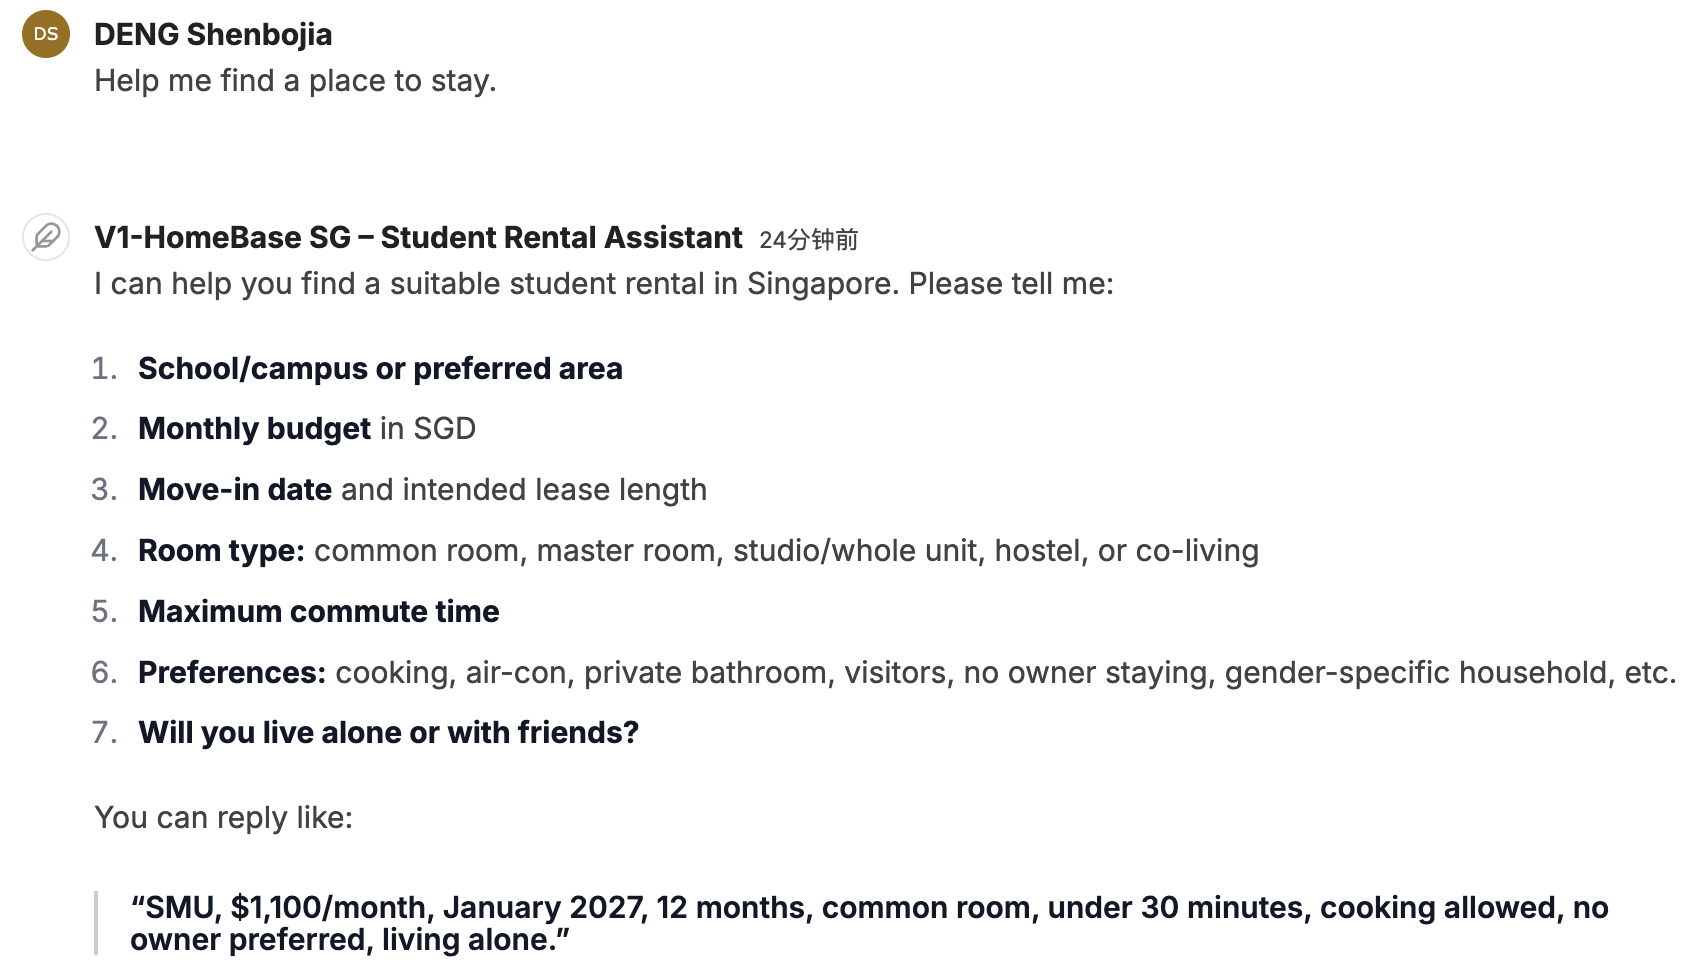
\includegraphics[width=\linewidth,height=5.5cm,keepaspectratio]{images/v1_test3.png}
\column{0.42\textwidth}
\centering\textbf{\textcolor{good}{After (V2): only 2 questions}}\\[3pt]
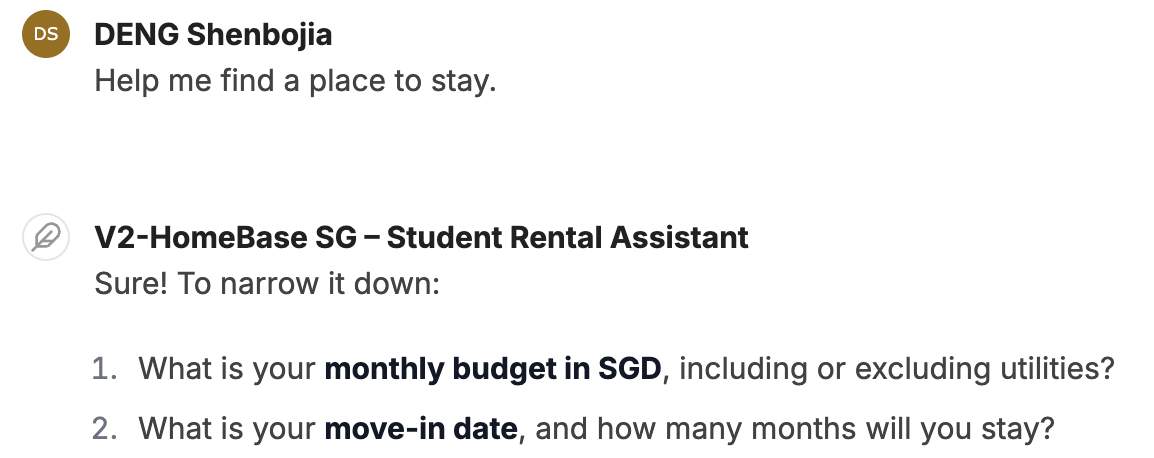
\includegraphics[width=\linewidth,height=5.5cm,keepaspectratio]{images/v2_test3.png}
\end{columns}
\vspace{4pt}
\textbf{Fix:} instruction \emph{``Start with easy questions, max 2 at a time.''} A long list can make a real student give up.
\end{frame}

% =====================================================================
\begin{frame}{Improvement 2: from one suggestion to a real comparison (Test 4)}
\footnotesize
\textbf{Prompt:} \emph{``I want somewhere very cheap but also within 10 minutes of SMU.''}\vspace{-4pt}

\begin{columns}[T]
\column{0.48\textwidth}
\centering\textbf{\textcolor{bad}{Before (V1): 1 option}}\\[3pt]
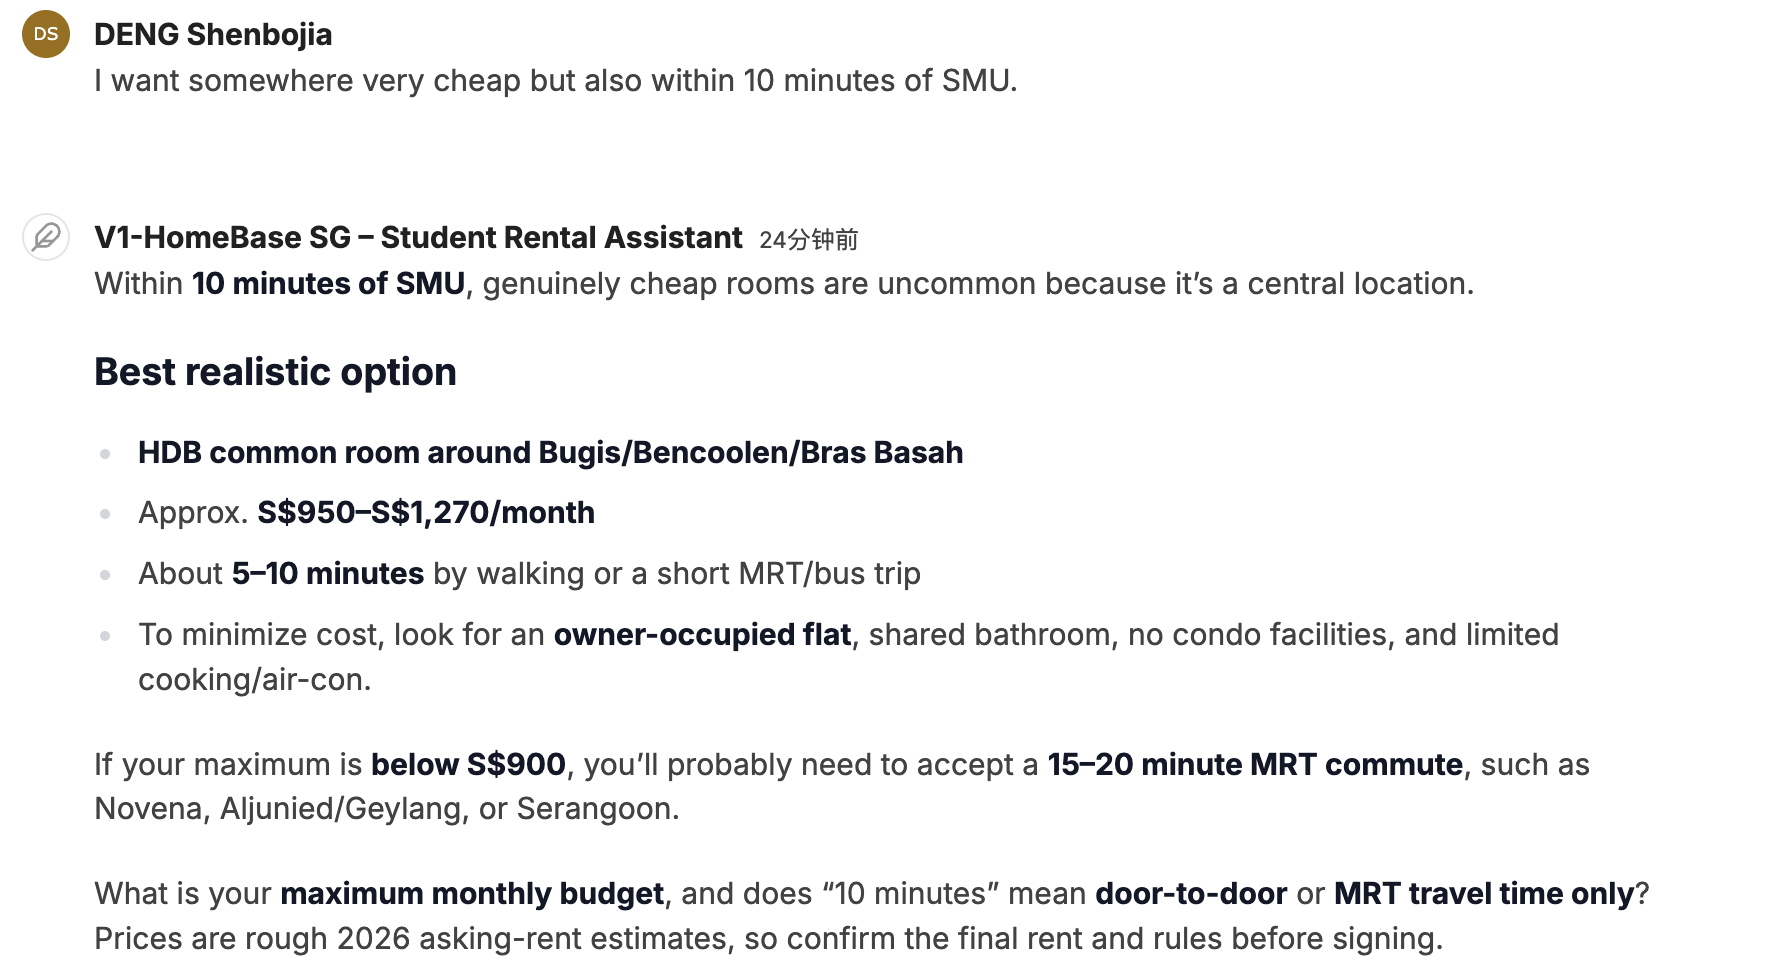
\includegraphics[width=\linewidth,height=5.5cm,keepaspectratio]{images/v1_test4.png}
\column{0.48\textwidth}
\centering\textbf{\textcolor{good}{After (V2): 3 options + trade-off}}\\[3pt]
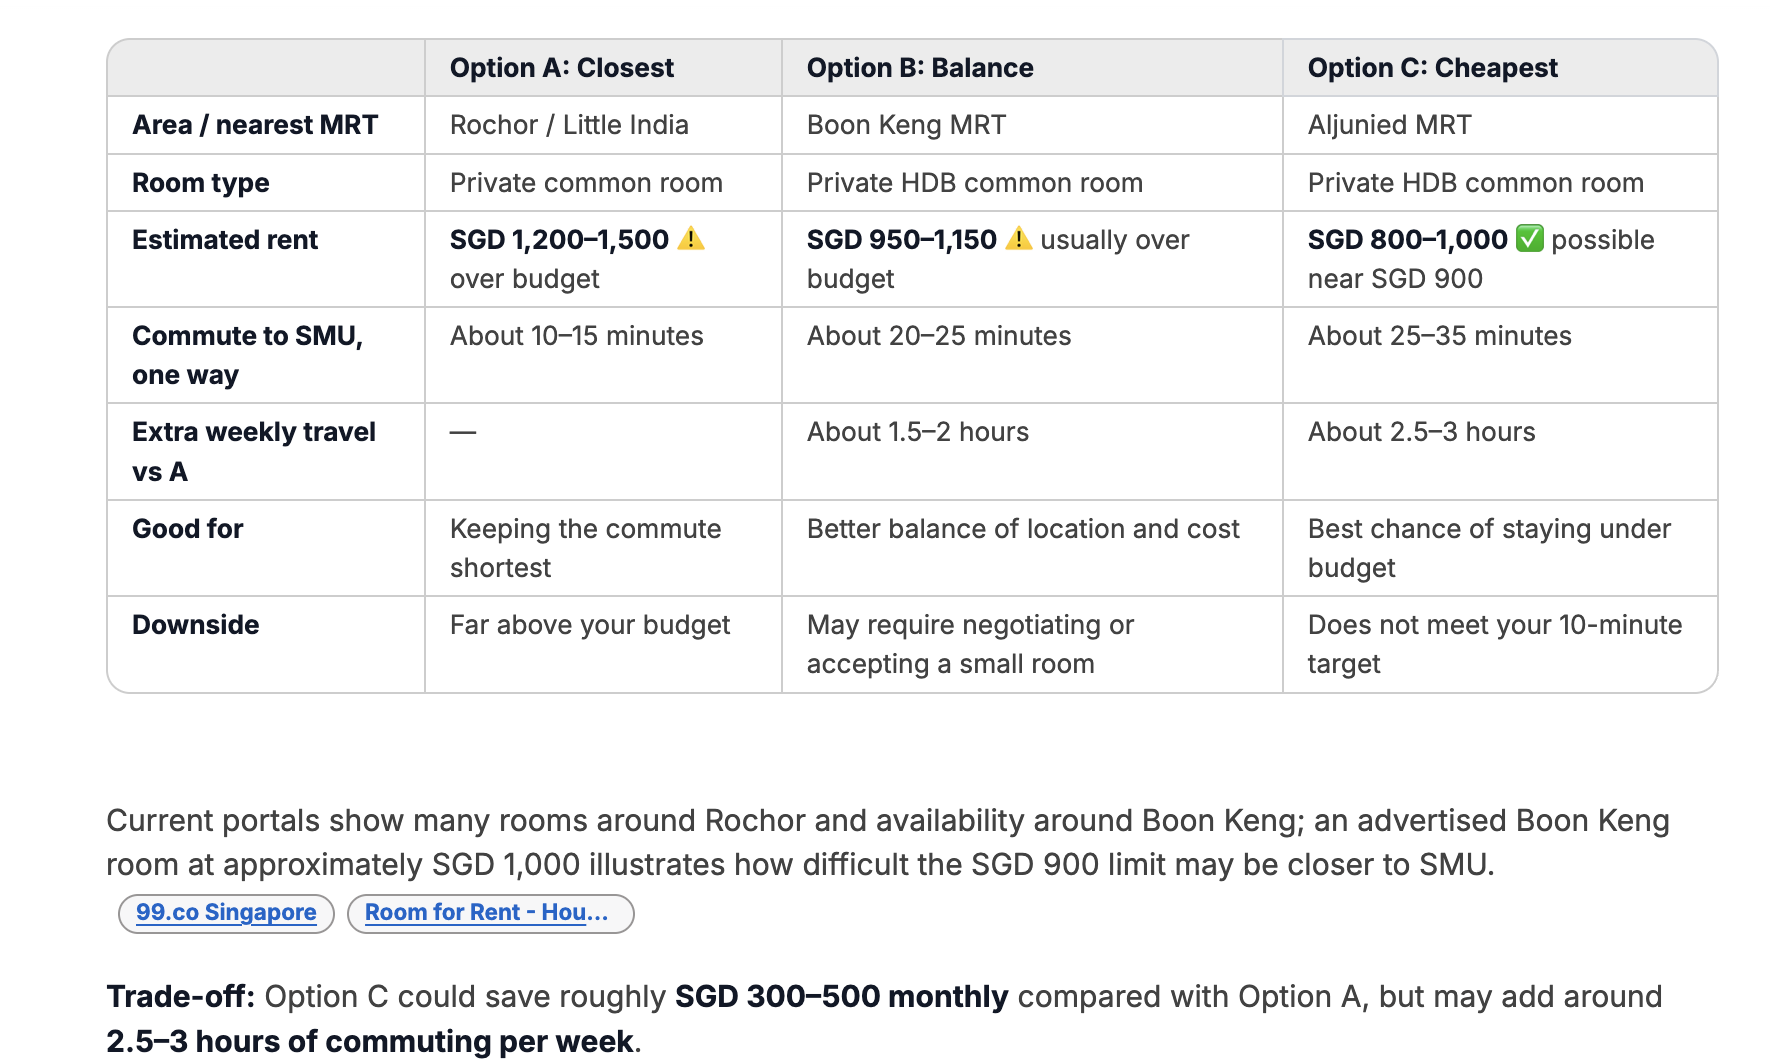
\includegraphics[width=\linewidth,height=5.5cm,keepaspectratio]{images/v2_test4.png}
\end{columns}
\vspace{4pt}
\textbf{Fix:} the \texttt{compare-rental-options} skill: 3 options, same table, trade-off in numbers, then ask what matters more.
\end{frame}

% =====================================================================
\begin{frame}[standout]
Live demo
\end{frame}

% =====================================================================
\begin{frame}{Limitations \& next steps}
\begin{columns}[T]
\column{0.48\textwidth}
\textbf{Limitations}
\begin{itemize}\footnotesize
  \item Rents are estimates, not live listings
  \item V2 sometimes asks 2 rounds of questions before giving options
  \item Rent figures did not always match our knowledge file (may use web results)
  \item Source links sometimes display wrongly (``Default'')
  \item V2 quoted one price from a search page with many prices: sounds more certain than it is
  \item No legal advice; built for SMU only
\end{itemize}
\column{0.48\textwidth}
\textbf{Next steps}
\begin{itemize}\footnotesize
  \item V3 rule: max 2 rounds of questions, then give options and state assumptions
  \item Tell the agent to use the knowledge file first for rents
  \item Connect to listing APIs for live data
  \item Hand-off to SMU housing staff
  \item Extend to other universities
\end{itemize}
\end{columns}
\end{frame}

% =====================================================================
\begin{frame}{Key takeaway}
\centering
\vspace{10pt}
{\Large \textcolor{purple}{\textbf{A focused agent}} that works well}\\[6pt]
{\Large matters more than}\\[6pt]
{\Large \textcolor{teal}{\textbf{a complicated agent}} with many features.}\\[18pt]
\normalsize HomeBase SG does two things well: \alert{help students choose} and \alert{keep them safe}.\\[14pt]
\Large Thank you! Questions?
\end{frame}

\end{document}
